\documentclass[10pt]{article}
\usepackage[russian]{babel}
\usepackage[utf8]{inputenc}
\usepackage[T2A]{fontenc}
\usepackage{amsmath}
\usepackage{amsfonts}
\usepackage{amssymb}
\usepackage[version=4]{mhchem}
\usepackage{stmaryrd}
\usepackage{graphicx}
\usepackage[export]{adjustbox}
\graphicspath{ {./images/} }

\begin{document}

\section*{Ангармоничность колебаний и генерация гармоник}

Как известно, в линейном консервативном осцилляторе, описываемом уравнением
\begin{equation}
\ddot{x} + \omega_0^2 x = 0, \tag{3.3}
\end{equation}

изменение во времени динамической переменной происходит по синусоидальному, или гармоническому закону:


\begin{equation*}
x=A \sin \left(\omega_{0} t+\varphi\right) \tag{3.4}
\end{equation*}


В нелинейной системе, совершающей периодические колебания, их форма обычно отличается от синусоиды. Такие колебания называют ангармоническими.

На рис. 3.9 показан вид временных зависимостей угла отклонения маятника при разной амплитуде колебаний. При малой амплитуде колебания близки к гармоническим. Это естественно, поскольку при малых углах отклонения маятник приближенно сводится к линейному осциллятору (3.3). Однако при больших амплитудах форма колебаний становится заметно отличной от синусоиды, т.е. колебания оказываются ангармоническими. «Глазомерный» способ различать гармонические и ангармонические колебания, конечно же, несовершенен. Чтобы придать этому различию более глубокий смысл и количественный аспект, необходимо обратиться к спектральному представлению колебаний.

Известно, что любую разумную с физической точки зрения периодическую функцию можно разложить в ряд Фурье. Путь $x(t)$ - функция периода $T$, тогда


\begin{equation*}
x(t)=\sum_{m=-\infty}^{\infty} c_{m} e^{2 \pi i m t / T} \tag{3.5}
\end{equation*}


где


\begin{equation*}
c_{m}=\frac{1}{T} \int_{0}^{T} x(t) e^{-2 \pi i m t / T} d t \tag{3.6}
\end{equation*}


Для того чтобы в любой момент $t$ величина $x(t)$ была действительной, коэффициенты разложения должны, очевидно, удовлетворять условию


\begin{equation*}
c_{m}=c_{-m}^{*}, \tag{3.7}
\end{equation*}


где звездочка обозначает комплексное сопряжение. Если мы сгруппируем члены ряда (3.5) по парам, отвечающим одинаковым по абсолютной величине значениям индекса $m$, то разложение Фурье можно записать в виде


\begin{equation*}
x(t)=A_{0}+\sum_{m=1}^{\infty} A_{m} \cos \left(m \omega t+\varphi_{m}\right) \tag{3.8}
\end{equation*}


где введены обозначения $\omega=2 \pi / T$ и


\begin{equation*}
A_{0}=c_{0}, A_{m}=\left|c_{m}\right|, \varphi_{m}=\arg c_{m} . \tag{3.9}
\end{equation*}


Полезное замечание о вычислении аргумента комплексного числа $x+i y$ : вместо общепринятого способа, когда полагают $\varphi=\operatorname{arctg}(y / x)$ при $x>0$ и $\varphi=\operatorname{arctg}(y / x)+\pi$ при $x<0$ можно рекомендовать более удобный эквивалентный способ, основанный на формуле


\begin{equation*}
\arg (x+i y)=2 \operatorname{arctg} \frac{y}{x+\sqrt{x^{2}+y^{2}}} . \tag{3.10}
\end{equation*}


Применение этой формулы не требует анализа того, в какую область попали $x$ и $y$.\\
(a)\\
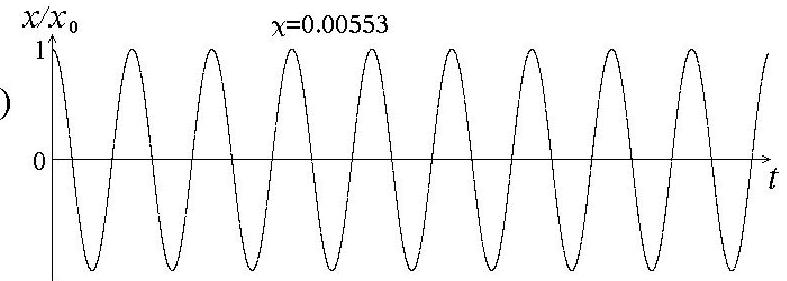
\includegraphics[max width=\textwidth, center]{2024_12_13_b73f3d6aa10f4b2a98e9g-043(2)}\\
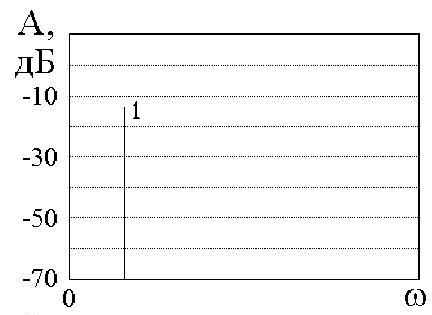
\includegraphics[max width=\textwidth, center]{2024_12_13_b73f3d6aa10f4b2a98e9g-043}\\
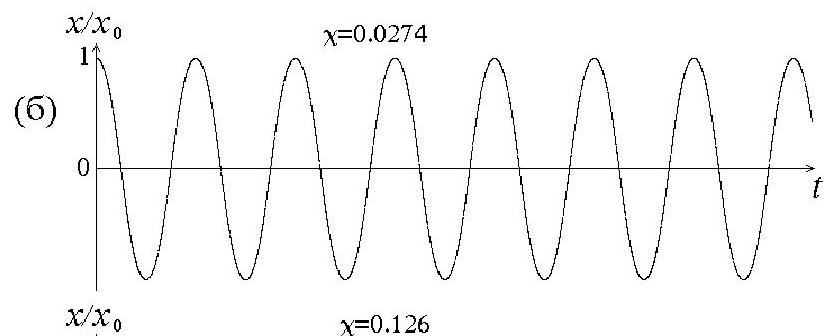
\includegraphics[max width=\textwidth, center]{2024_12_13_b73f3d6aa10f4b2a98e9g-043(3)}\\
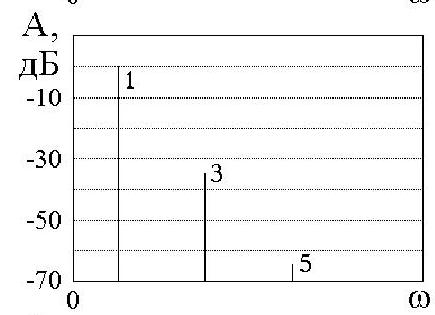
\includegraphics[max width=\textwidth, center]{2024_12_13_b73f3d6aa10f4b2a98e9g-043(5)}\\
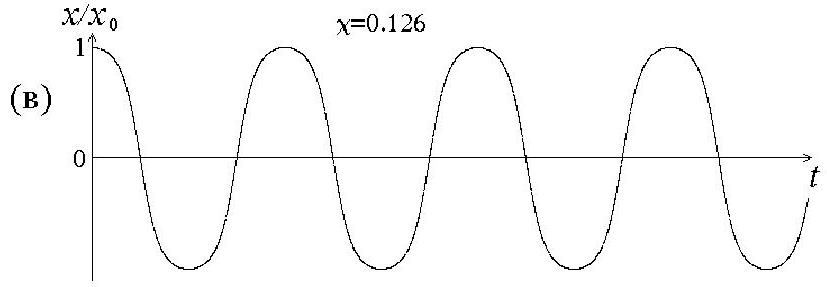
\includegraphics[max width=\textwidth, center]{2024_12_13_b73f3d6aa10f4b2a98e9g-043(4)}\\
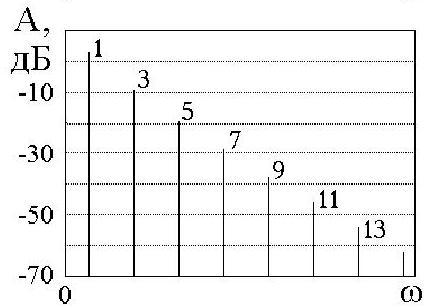
\includegraphics[max width=\textwidth, center]{2024_12_13_b73f3d6aa10f4b2a98e9g-043(1)}

Рис. 3.9. Справа - зависимости угловой координаты маятника от времени при начальном отклонении, соответственно, $x_{0}=1$ (a), 2 (б) и 3(в), указаны числовые значения коэффициента нелинейных искажений. Справа - соответствующие спектры, где по оси ординат использован логарифмический масштаб, и амплитуды гармоник даны в децибелах. Цифрами обозначены номера гармоник, обратите внимание, что присутствуют только нечетные гармоники. Графики получены путем численного решения уравнения динамики маятника на компьютере.

Член ряда (3.8) с нулевым индексом отвечает постоянной составляющей, которую часто целесообразно бывает исключить из рассмотрения надлежащим выбором начала отсчета для динамической переменной $x$. Если отличен от нуля один только первый член суммы, то это соответствует гармоническим колебаниям, которые, с общей точки зрения, представляют собой очень специальный случай периодического колебательного процесса. Если же сумма содержит другие ненулевые члены, то колебания ангармонические, поскольку их форма с очевидностью отличается от простой синусоиды. Чаще всего самую большую амплитуду имеет первый член $A_{1} \cos \left(\omega t+\varphi_{1}\right)$. Его считают ос-

новной гармонической составляющей процесса, и говорят о ней как о первой гармонике. Последующие члены ряда отвечают второй гармонике $A_{2} \cos \left(2 \omega t+\varphi_{2}\right)$, третьей гармонике $A_{3} \cos \left(3 \omega t+\varphi_{3}\right)$ и т.д. Очевидно, частота колебаний $m$-ой гармоники равна $m \omega$.

В качестве количественной характеристики отклонения колебательного процесса от гармонических колебаний в технике используют так называемый коэффициент нелинейных искажений. Он определяется как отношение


\begin{equation*}
\chi=\frac{\sqrt{A_{2}^{2}+A_{3}^{2}+A_{4}^{2}+A_{5}^{2}+\ldots}}{A_{1}} \tag{3.11}
\end{equation*}


Итак, со спектральной точки зрения, отличие колебаний по форме от синусоиды ангармоничность трактуется как присутствие составляющих с частотами $2 \omega, 3 \omega, \ldots$, высших гармоник. Вопрос о происхождении ангармоничности есть вопрос о причине возникновения (генерации) высших гармоник. Если представить колебательную систему построенной из отдельных составных элементов, то появление высших гармоник можно связать с преобразованием спектра периодического сигнала нелинейными элементами. Обсудим подробнее этот простой, но важный для теории колебаний общий принцип.

Пусть мы имеем элемент, для которого входной сигнал дается переменной $x(t)$, выходной - переменной $y(t)$, а связывающая их нелинейная характеристика раскладывается в ряд Тейлора


\begin{equation*}
y=a_{1} x+a_{2} x^{2}+a_{3} x^{3}+\ldots \tag{3.12}
\end{equation*}


Первый член в этом разложении линейный, второй и третий представляют, как говорят, квадратичную и кубическую нелинейность, соответственно.

Предположим, что входной сигнал гармонический, $x(t)=A \sin (\omega t+\varphi)$, т.е. в спектре присутствует только одна частотная составляющая, на частоте $\omega$. Подставим выражение для $x(t)$ в (3.12). При помощи известных тригонометрических формул степени синуса могут быть представлены в виде линейных комбинаций гармонических функций. В силу того, что


\begin{equation*}
\sin ^{2} \alpha=\frac{1}{2}-\frac{1}{2} \cos 2 \alpha=\frac{1}{2}+\frac{1}{2} \sin \left(2 \alpha-\frac{\pi}{2}\right), \tag{3.13}
\end{equation*}


член, отвечающий за квадратичную нелинейность, принимает вид


\begin{align*}
& a_{2} A^{2} \sin ^{2}(\omega t+\varphi)=\frac{1}{2} a_{2} A^{2}(1-\cos (2 \omega t+2 \varphi))  \tag{3.14}\\
& \quad=\frac{1}{2} a_{2} A^{2}+\frac{1}{2} a_{2} A^{2} \sin \left(2 \omega t+2 \varphi-\frac{\pi}{2}\right)
\end{align*}


Далее, поскольку


\begin{equation*}
\sin ^{3} \alpha=\frac{3}{4} \sin \alpha-\frac{1}{4} \sin 3 \alpha, \tag{3.15}
\end{equation*}


то член, соответствующий кубической нелинейности, переписывается в виде


\begin{equation*}
A^{3} \sin ^{3}(\omega t+\varphi)=\frac{3}{4} a_{3} A^{3} \sin (\omega t+\varphi)+\frac{1}{4} a_{3} A^{3} \sin (3 \omega t+3 \varphi+\pi) . \tag{3.16}
\end{equation*}


Собирая все члены, имеем окончательно:


\begin{align*}
& y=\frac{1}{2} a_{2} A^{2}+\left(a_{1} A+\frac{3}{4} a_{3} A^{3}\right) \sin (\omega t+\varphi)+\frac{1}{2} a_{2} A^{2} \sin \left(2 \omega t+2 \varphi-\frac{\pi}{2}\right) \\
& +\frac{1}{4} \sin (3 \omega t+3 \varphi+\pi)+\ldots \tag{3.17}
\end{align*}


Из проведенных простых выкладок видно, что присутствие на выходе нелинейного элемента гармонических составляющих с частотами, отличными от частоты входного сигнала, обязано нелинейности характеристики элемента (рис. 3.10). При этом квадратичная нелинейность отвечает за появление постоянной составляющей (в радиотехнике об этом эффекте говорят как о детектировании) и второй гармоники. Обратите внимание, что соответствующие слагаемые в формуле (3.17) пропорциональны коэффициенту квадратичной нелинейности $a_{2}$ и квадрату входной амплитуды. Кубическая нелинейность обеспечивает нелинейную добавку к амплитуде основной гармоники и возникновение третьей гармоники. Заметьте, что соответствующие слагаемые пропорциональны коэффициенту кубической нелинейности $a_{3}$ и кубу входной амплитуды.

Одной из красивейших иллюстрацией нелинейного преобразования частот служит следующий оптический эксперимент. Луч электромагнитного излучения инфракрасного диапазона, невидимый глазом (длина волны 1,06 мкм, частота $2,8 \cdot 10^{14}$ Гц), генерируется лазером на неодимовом стекле и проходит через кристалл ниобата бария. При достаточно большой интенсивности в результате нелинейного квадратичного преобразования электромагнитных колебаний в кристалле генерируется вторая гармоника с частотой вдвое больше исходной, 5,6 $\cdot 10^{14}$ Гц. Эта частота соответствует уже видимому диапазону оптического излучения, и на выходе из кристалла наблюдается луч зеленого цвета (длина волны 0,53 мкм). Аналогичный эффект наблюдается в акустике. Имея источник достаточно интенсивный источник звука определенной частоты $f_{0}$ можно обнаружить, что на достаточно большом расстоянии от источника акустические колебания содержат вторую, третью и другие гармоники, т.е. составляющие с частотами $2 f_{0}$, $3 f_{0}$ и т.д. Их можно фиксировать с помощью аппаратуры или воспринять на слух. Еще один пример относится к физиологии слуха. Как обнаружено в свое время Гельмгольцем, генерация гармоник сопровождает собственно процесс восприятия ухом монохроматического звука при его большой амплитуде. (При этом, чтобы различить высшие гармоники на фоне интенсивного основного тона нужно обладать достаточно тренированным музыкальным слухом!)


\end{document}